\documentclass[10pt,a4paper]{article}
\usepackage[utf8]{inputenc}
\usepackage{amsmath}
\usepackage{amsfonts}
\usepackage{amssymb}
\usepackage{amsthm}
\usepackage{float}
\usepackage{mathtools}
\usepackage{geometry}[margin=1in]
\usepackage{xspace}
\usepackage{tikz}
\usepackage{mathrsfs}
\usetikzlibrary{shapes, arrows, decorations.pathmorphing}
\usepackage[parfill]{parskip}
\usepackage{subcaption}
\usepackage{stmaryrd}
\usepackage{marvosym}
\usepackage{dsfont}

\newcommand{\st}{\text{ s.t. }}
\newcommand{\contr}{\lightning}
\newcommand{\im}{\mathfrak{i}}
\newcommand{\R}{\mathbb{R}}
\newcommand{\Q}{\mathbb{Q}}
\newcommand{\C}{\mathbb{C}}
\newcommand{\F}{\mathbb{F}}
\newcommand{\K}{\mathbb{K}}
\newcommand{\N}{\mathbb{N}}
\newcommand{\Z}{\mathbb{Z}}
\renewcommand{\H}{\mathds{H}}
\newcommand{\nequiv}{\not\equiv}
\newcommand{\powset}{\mathcal{P}}
\renewcommand{\th}[1][th]{\textsuperscript{#1}\xspace}
\newcommand{\from}{\leftarrow}
\newcommand{\legendre}[2]{\left(\frac{#1}{#2}\right)}
\newcommand{\ow}{\text{otherwise}}
\newcommand{\imp}[2]{\underline{\textit{#1.}$\implies$\textit{#2.}}}
\let\oldexists\exists
\renewcommand{\exists}{\oldexists\;}
\renewcommand{\hat}{\widehat}
\renewcommand{\tilde}{\widetilde}
\newcommand{\one}{\mathds{1}}
\newcommand{\under}{\backslash}
\newcommand{\injection}{\hookrightarrow}
\newcommand{\surjection}{\twoheadrightarrow}
\newcommand{\jacobi}{\legendre}
\newcommand{\floor}[1]{\lfloor #1 \rfloor}
\newcommand{\ceil}[1]{\lceil #1 \rceil}
\newcommand{\cbrt}[1]{\sqrt[3]{#1}}

\DeclareMathOperator{\ex}{ex}
\DeclareMathOperator{\id}{id}
\DeclareMathOperator{\upper}{Upper}
\DeclareMathOperator{\dom}{dom}

\DeclareMathOperator{\charr}{char}
\DeclareMathOperator{\Image}{im}
\DeclareMathOperator{\ord}{ord}
\DeclareMathOperator{\lcm}{lcm}
\let\emph\relax
\DeclareTextFontCommand{\emph}{\bfseries\em}

\newtheorem{theorem}{Theorem}[section]
\newtheorem{lemma}[theorem]{Lemma}
\newtheorem{corollary}[theorem]{Corollary}
\newtheorem{proposition}[theorem]{Proposition}
\newtheorem{conjecture}[theorem]{Conjecture}

\tikzset{sketch/.style={decorate,
 decoration={random steps, amplitude=1pt, segment length=5pt}, 
 line join=round, draw=black!80, very thick, fill=#1
}}

\title{Coding \& Cryptography}
\begin{document}
\maketitle

\setcounter{section}{-1}
\section{Communication Channels}
This course will be about modelling communication. In general, we have the following idea:

\begin{figure}[H]
\centering

\begin{tikzpicture}
\node (s) at (0,0) {\textsc{Source}};
\node (e) at (4,0) {\textsc{Encoder}};
\node (d) at (8,0) {\textsc{Decoder}};
\node (r) at (12,0) {\textsc{Receiver}};
\draw (s) edge[->] (e) (d) edge[->] (r);
\draw[->, decorate, line join=round, decoration={zigzag, segment length=4, amplitude=0.9, post=lineto, post length=2pt}] (e) -- node[above] {\textsc{Channel}} node[below] {Errors, Noise} (d) ;
\end{tikzpicture}
\end{figure}
\vspace{-1em}
For example, the channel might be an optical or electrical telegraph, modems, audio CDs, satellite relays. The encoding and decoding might be something like \textsc{Ascii}, so that each character in the email ``Call at 2pm" would be encoded into 8 bits using $a = 1100101, \ldots$, giving an 84 bit message to be transmitted via the internet, and decoded by the receiver's email client. Our general aim here will be, given some source and channel (modelled probabilistically), to design an encoder and decoder to send messages economically and reliably.

\underline{Examples}
\begin{itemize}
\item (Noiseless coding) Morse Code. In this code, more common letters are assigned shorter codes, so that we have $A = \cdot - \ast, E = \cdot \ast, Q = - - \cdot - \ast, Z = - - \cdot \cdot \ast$. This is adapted to the \textit{source}, in the sense that we chose the codes based off the expected distribution of letters that we will have to transmit.

\item (Noisy coding) \textsc{Isbn}. In the \textsc{Isbn} encoding, every book is given a 10 digit number $a_1a_2\ldots a_{10}$, with $\sum_{i=1}^{10} (11-i)a_i \equiv 0 \mod 11$. This is adapted to the \textit{channel}, in the sense that the likely errors to occur will be 1 incorrect digit, or accidentally transposing two digits, which this code is resistant to (will return an error rather than an erroneous result).
\end{itemize}

A \emph{communication channel} accepts symbols from some alphabet $\mathcal{A} = \{a_1, a_2, \ldots, a_r\}$ (e.g. $\{0,1\}, \{a,b,\ldots,z\}$), and outputs symbols from an alphabet $\mathcal{B} = \{b_1, \ldots, b_s\}$. The channel is modelled by the probabilities:
\begin{center}$\P(y_1,y_2,\ldots,y_n$ received$| x_1,x_2,\ldots,x_n$ sent$) = \prod_{i=1}^{n} \P(y_i$ received$| x_i$ sent$)$\end{center}

A \emph{discrete memoryless channel (DMC)} is a channel with $p_{ij} = \P(b_j$ received$|a_i$ sent$)$ the same for each channel usage and independent of any past or future channel usages.

The \emph{channel matrix} is $P = (p_{ij})$, an $r \times s$ stochastic matrix.

\underline{Examples:} The \emph{binary symmetric channel (BSC)} with error probability $p \in [0,1]$ has $\mathcal{A} = \mathcal{B} = \{0,1\}$. The channel matrix is $\begin{pmatrix} 1-p & p \\ p & 1-p \end{pmatrix}$. A symbol is transmitted correctly with probability $1-p$.

The \emph{binary erasure channel} has input alphabet $\{0,1\}$, and output alphabet $\{0, 1, \ast\}$, where we miss a bit is probability $p$, giving channel matrix $\begin{pmatrix} 1-p & 0 & p \\ 0 & 1-p & 0\end{pmatrix}$. We can model $n$ uses of a channel by the \emph{n\th extension} with input alphabet $\mathcal{A}^n$, and output alphabet $\mathcal{B}^n$.

A \emph{code} $c$ of \emph{length} $n$ is a function $c: M \to \mathcal{A}^n$ where $M$ is the set of all possible messages. Implicitly, we also have a decoding rule $\mathcal{B}^n \to M$.\\
The \emph{size} of $c$ is $m = |M|$. \\
The \emph{information rate} is $\rho(c) = \frac{1}{n}\log_2(m)$. \\
The \emph{error rate} is $\hat{e}(c) = \max_{x\in M} \{\P($error$|x$ sent$)\}$.

A channel can transmit reliably at a rate $R$ if there exists a sequence of codes $(c_n: n\geq 1)$ with $c_n$ a code of length $n$, $\lim_{n\to \infty}(\rho(c_n)) =R, \lim_{n\to\infty}(\hat{e}(c_n)) = 0$. The capacity of a channel is the supremum of all reliable transmission rates.

\begin{theorem}
A $BSC$ with error probability $p < \frac12$ has a non-zero capacity (i.e. good codes exist).
\end{theorem}
\begin{proof}
See \textbf{9.3}
\end{proof}

\section{Noiseless Coding}
\subsection{Prefix-free Codes}
For an alphabet $\mathcal{A}, |\mathcal{A}|<\infty$, let $\mathcal{A}^{\ast} = \bigcup_{n\geq 0} \mathcal{A}^n$, the set of all finite strings from $\mathcal{A}$. The \emph{concatenation} of strings $x = x_1\ldots x_r$ and $y = y_1\ldots y_s$ is $xy = x_1\ldots x_ry_1\ldots y_s$.

Let $\mathcal{A}, \mathcal{B}$, be alphabets. A \emph{code} is a function $c:\mathcal{A} \to \mathcal{B}^{\ast}$. The strings $c(a)$ for $a \in \mathcal{A}$ are called \emph{codewords} (cws). If $x, y \in \mathcal{B}^{\ast}$ then $x$ is a \emph{prefix} of $y$ if $y=xz$ for some $z \in \mathcal{B}^{\ast}$.

For example, we have the Greek fire code, found in the writings of Polybius around 280 BC. $\mathcal{A} = \{\alpha, \beta, \ldots, \omega\}, \mathcal{B} = \{1,2,3,4,5\}$, with code $\alpha \mapsto 11, \beta \mapsto 12, \ldots, \psi \mapsto 53, \omega \mapsto, 54$, where $xy$ means ``$x$ torches held up, and another $y$ torches nearby".

The English language is even a code: we can let $\mathcal{A}$ be words in a given dictionary, and $\mathcal{B} = \{a,b,\ldots,z,\text{\textvisiblespace}\}$, where the coding function is to spell the word and follow it with a space.

We send a message $x_1\ldots x_n \in \mathcal{A}^{\ast}$ as $c(x_1)\ldots c(x_n) \in \mathcal{B}^{\ast}$. So $c$ extends to a function $c^{\ast}:\mathcal{A}^{\ast} \to \mathcal{B}^{\ast}$.

$c$ is \emph{decipherable}/\emph{decidable} if $c^{\ast}$ is injective, so that each string in $\mathcal{B}^{\ast}$ could have come from at most one message. Note that it isn't sufficient to just have $c$ injective, although clearly this is necessary:

$\mathcal{A} = \{1,2,3,4\}, \mathcal{B} = \{0,1\}, c:1\mapsto 0, 2\mapsto 1, 3\mapsto 00, 4\mapsto 01$. Then $c^{\ast}(114) = 0001 = c^{\ast}(312)$.

If $|\mathcal{A}|=m, |\mathcal{B}|=a$, then we say $c$ is an \emph{a-ary code of size m}. 2-ary = \emph{binary}, 3-ary=\emph{ternary}.

We aim to construct decipherable codes with short word lengths. Assuming $c$ is injective, the following are always decipherable:
\begin{itemize}
\item Block codes, where every codeword has the same length (e.g. Greek fire, \textsc{Ascii})
\item Comma codes, where we have an ``end of word" character (e.g. English language)
\item Prefix-free codes, where no codeword is a prefix of any other distinct words.
\end{itemize}
Note that both of the first two are special cases of prefix-free codes. Prefix-free codes are often called \emph{instantaneous} or \emph{self-punctuating} codes. Note that not all decipherable codes are prefix-free: $0\mapsto 01, 1 \mapsto 011$ is decipherable but not prefix free.

\begin{theorem}[Kraft's Inequality]
Let $|\mathcal{A}| = m, |\mathcal{B}| = a$. A prefix-free code $c:\mathcal{A} \to \mathcal{B}^{\ast}$ with word lengths $\ell_1, \ldots, \ell_m$ exists if and only if:
\begin{align*}
\sum_{i=1}^{m} a^{-\ell_i} &\leq 1 \tag{\ast}
\end{align*}
\end{theorem}
\begin{proof}
Rewrite (\ast) as $\sum_{\ell=1}^s n_{\ell}a^{-\ell} \leq 1 (\star)$, where $n_{\ell}$ is the number of codewords of length $\ell$ and $s = \max_{1 \leq i \leq m} \ell_i$.

\begin{itemize}
\item[$\implies$] If $c:\mathcal{A} \to \mathcal{B}^{\ast}$ is prefix-free, then $n_1 a^{s-1} + n_2 a^{s-2} + \ldots n_s \leq a^s$, since the \textsc{Lhs} is the number of strings of length $s$ in $\mathcal{B}$ with some codeword of $c$ as a prefix, and \textsc{Rhs} is the number of strings of length $s$. Dividing by $a^{s}$ gives $(\star)$.

\item[$\impliedby$] Given $n_1, \ldots, n_s$ satisfying $(\star)$, we need to construct a prefix-free code $c$ with $n_\ell$ codewords of length $\ell$ for all $\ell \leq s$. We use induction on $s$. The case $s=1$ is clear: we have $(\star)$ gives $n_1 \leq a$, so we can choose a code.

By the induction hypothesis there is a prefix-free code $\hat{c}$ with $n_{\ell}$ codewords of length $\ell$ for all $\ell \leq s-1$. Then $(\star)$ gives:
\begin{align*}
n_1 a^{s-1} + n_2 a^{s-2} + \ldots + n_{s-1}a + n_s &\leq a^s
\end{align*}
where the first $s-1$ terms on \textsc{Lhs} sum to the number of strings of length $s$ with some codeword of $\hat{c}$ as a prefix, and the \textsc{Rhs} is the number of strings of length $s$. Hence we can add at least $n_s$ new codewords of length $s$ to $\hat{c}$ and maintain the prefix-free property, giving our code.
\end{itemize}
\end{proof}

\begin{theorem}[McMillan]
Any decipherable code satisfies Kraft's inequality
\end{theorem}
\begin{proof}[Karush]
Let $c:\mathcal{A} \to \mathcal{B}^{\ast}$ be a decipherable code with codewords of lengths $\ell_1, \ldots, \ell_m$. Let $s = \max_{1 \leq i\leq m} \ell_i$. Then for $R \in \N:$
\begin{align*}
\left(\sum_{i=1}^{m} a^{-\ell_i}\right)^R = \sum_{l=1}^{Rs} b_{\ell}a^{-\ell}
\end{align*}
where $b_{\ell} = |\{x \in \mathcal{A}^R : c^{\ast}(x)$ has length $\ell\}| \leq |\mathcal{B}^{\ell}| = a^{\ell}$, using the fact that $c^{\ast}$ is injective. Then:
\begin{align*}
\left(\sum_{i=1}^m a^{-\ell_i}\right)^R &\leq \sum_{l=1}^R a^\ell a^{-\ell} = Rs\\
\sum_{i=1}^m a^{-\ell_i} &\leq (Rs)^{\frac1R} \to 1 \text{ as } R \to \infty
\end{align*}
\end{proof}

\begin{corollary}
A decipherable code with prescribed word lengths exists iff a prefix-free code with same word lengths exists.
\end{corollary}
\begin{proof}
\item
\begin{itemize}
\item[$\implies$] Use \textbf{1.2} to generate a prefix-free code by \textbf{1.1}
\item[$\impliedby$] Prefix-free codes are decipherable.
\end{itemize}
\end{proof}

\section{Shannon's Noiseless Coding Theorem}
Entropy is a measure of `randomness' or `uncertainty'. Suppose we have a random variable $X$ that takes values $x_1, \ldots, x_n$ with probabilities $p_1, \ldots, p_n$. Then the \emph{entropy} (roughly speaking) is the expected number of fair coin tosses needed to simulate $X$.

\hspace*{-1em}\underline{Examples:}
\begin{itemize}
\item $p_1 = p_2 = p_3 = p_4 = \frac14$. We can identify $\{x_1, x_2, x_3, x_4\}$ with $\{HH, HT, TH, TT\}$, and so the entropy of this random variable is $2$.

\item $(p_1, p_2, p_3, p_4)=(\frac12,\frac14,\frac18,\frac18)$. Here, the entropy is $1\cdot\frac12+2\cdot\frac14+3\cdot\frac18+3\cdot\frac18 = \frac74$. We might say then, since the entropy is greater, that the first example is ``more random" than the second.
\end{itemize}

More concretely, the \emph{Shannon (or information) entropy} of $X$ is $H(X) = -\sum_{i=1}^n p_i \log_2 p_i$. Note that $H(X) \geq 0$ with equality if and only if $\P(X=x_i) = 1$. This is measured in \emph{bits}. We take the convention that $0\log 0 =0$.

\hspace*{-1em}\underline{Example}: Consider a biased coin, where $\P(X=H) = p, \P(X=T) = 1-p$. Then $H(X) = -p\log p-(1-p)\log(1-p) = p\log(\frac{1-p}{p} - \log(1-p)$.

\begin{figure}[H]
\centering
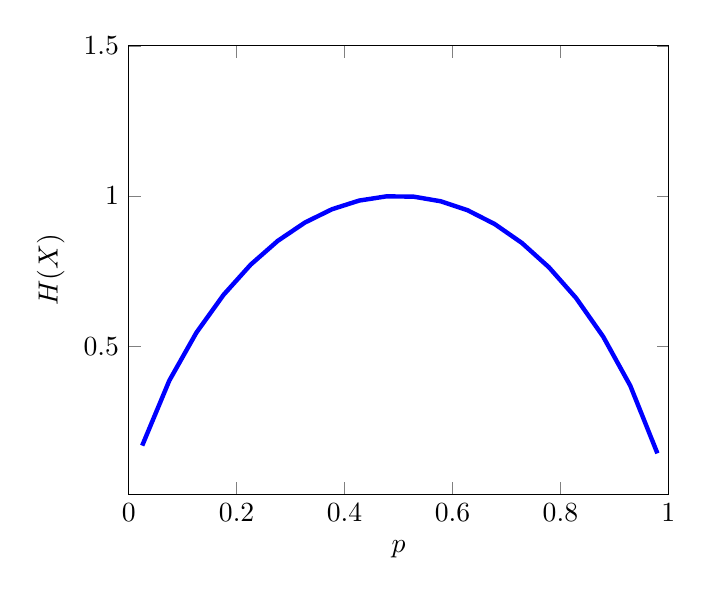
\begin{tikzpicture}
\begin{axis}[xmin=0, xmax=1 ,ymax=1.5, samples=50, xlabel = {$p$}, ylabel={$H(X)$}]
\addplot[blue, ultra thick, samples=200] (x, {x*log2((1-x)/x) - log2(1-x)});
\end{axis}
\end{tikzpicture}
\end{figure}

\begin{proposition}[Gibb's Inequality]
Let $(p_1, \ldots, p_n)$ and $(q_1, \ldots, q_n)$ be probability distributions. Then:
\begin{align*}
-\sum_{i=1}^n p_i \log p_i \leq -\sum_{i=1}^n p_i \log q_i
\end{align*}
with equality if and only if $p_i = q_i$ for all $i$.
\end{proposition}

\begin{proof}
Since $\log x = \frac{\ln x}{\ln 2}$, we may replace $\log$ by $\ln$ in the proof. Put $I = \{1 \leq r\leq n: p_i \neq 0\}$. Now $\ln x \leq x-1$ with equality if and only if $x=1$. So we have $\ln \frac{q_i}{p_i} \leq \frac{q_i}{p_i} - 1$, and hence:
\begin{align*}
\sum_{i \in I} p_i \ln \frac{q_i}{p_i} &\leq \sum_{i\in I}q_i - \sum_{i \in I}p_i\\
&= \sum_{i \in I} q_i - 1 \leq 0\\
\therefore - \sum_{i \in I}p_i \ln p_i &\leq - \sum_{i \in I} p_i \ln q_i\\
\therefore -\sum_{i=1}^n p_i \log p_i &\leq -\sum_{i=1}^n p_i \log q_i
\end{align*}
If equality holds, then $\sum_{i\in I} p_i =1$ and $\frac{p_i}{q_i} = 1$ for all $i \in I$, so $p_i = q_i$
\end{proof}

\begin{corollary}
$H(p_1, \ldots, p_n) \leq \log n$ with equality if and only if $p_1 = \ldots = p_n = \frac1n$.
\end{corollary}
\begin{proof}
Take $q_1 = \ldots = q_n = \frac1n$ in \textbf{2.1}.
\end{proof}

Let $\mathcal{A} = \{\mu_1, \ldots, \mu_m\}$, and $|\mathcal{B}| = a$, where $m, a\geq 2$. The random variable $X$ takes values $\mu_1, \ldots, \mu_m$ with probabilities $p_1, \ldots, p_m$. We say a code $c:\mathcal{A} \to \mathcal{B}^{\ast}$ is \emph{optimal} if it is a decipherable code with smallest possible expected word length, $\E S = \sum_i p_i \ell_i$.

\begin{theorem}[Shannon's Noiseless Coding Theorem]
The expected word length $\E S$ of an optimal code satisfies:
\begin{align*}
\frac{H(X)}{\log a} \leq \E S < \frac{H(X)}{\log a}+1
\end{align*}
\end{theorem}
\begin{proof}
For the lower bound, take $c: \mathcal{A} \to \mathcal{B}^{\ast}$ decipherable with word lengths $\ell_1, \ldots, \ell_m$. Then set $q_i = \frac{a^{-\ell_i}}{D}$ where $D = \sum_{i=1}^m a^{-\ell_i}$. Now we have that $\sum_{i=1}^m q_i = 1$. By Gibbs,
\begin{align*}
H(X) &\leq -\sum_{i=1}^m p_i \log q_i\\
&= -\sum p_i\left(-\ell_i \log a - \log D\right)\\
&= \left(\sum_{i=1}^m p_i \ell_i\right) \log a + \log D
\end{align*}
By McMillan, $D \leq 1$, so $\log D \leq 0$, and so $H(X) \leq \left(\sum_{i=1}^m p_i \ell_i\right) \log a = \E S \cdot \log a$, and we have equality if and only if $p_i = a^{-\ell_i}$ for some integers $\ell_1, \ldots \ell_m$.

For the upper bound, take $\ell_i = \ceil{-\log_a p_i}$. Then $-\log_a p_i \leq \ell_i \implies p_i \geq a^{-\ell_i}$.

Now $\sum_{i=1}^m a^{-\ell_i} \leq \sum_{i=1}^m p_i = 1$. By Kraft, there is some prefix-free code $c$ with word lengths $\ell_1, \ldots, \ell_m$, and the expected word length of $c$ is $\E S = \sum p_i \ell_i < \sum p_i (-\log_a p_i + 1) = \frac{H(X)}{\log a} + 1$.
\end{proof}

\hspace*{-1em}\underline{Example:} \emph{Shannon-Fano coding}\\
We mimic the above proof: given probabilities $p_1, \ldots, p_n$, set $\ell_i = \ceil{-\log_a p_i}$. Construct the prefix-free code with word lengths $\ell_1, \ldots, \ell_m$ by choosing in order of increasing length, ensuring that previous codewords are not prefixes. For example, if $a = 2, m = 5$ we have:\\
\begin{figure}[H]
\centering
\begin{tabular}{c|c|c|c}
$i$ & $p_i$ & $\ceil{-\log_2 p_i}$ & Codewords \\\hline
1 & 0.4 & 2 & 00 \\
2 & 0.2 & 3 & 010\\
3 & 0.2 & 3 & 011\\
4 & 0.1 & 4 & 1000\\
5 & 0.1 & 4 & 1001
\end{tabular}
\end{figure}
$\E S = \sum p_i \ell_i = 2.8$, entropy $= 2.12$

\section{Huffman Coding Algorithm}
Huffman was a student of Fano, and was thinking about how to construct an optimal code. For simplicity, we will take $a = 2$. Suppose we get messages with orders $p_1 \geq p_2 \geq \ldots \geq p_m$. Huffman gave a recursive definition of codes that we can prove are optimal. If $m=2$, then take codewords $0$ and $1$.

If $m > 2$, we first have a Huffman code for messages $\mu_1, \ldots, \mu_{m-2}, \nu$ with probabilities $p_1, \ldots, p_{m-2}, p_{m-1}+p_m$, then append $0$ and $1$ to give codewords for $\mu_{m-1}$ and $\mu_m$.

\hspace*{-1em}Note:
\begin{itemize}
\item Huffman codes are prefix-free.
\item We have some choices to make if some of the $p_j$ are equal, so Huffman codes are not unique.
\end{itemize}
\hspace*{-1em}\underline{Example:} Reconsider the previous example:
\begin{figure}[H]
\begin{subfigure}{0.5\textwidth}
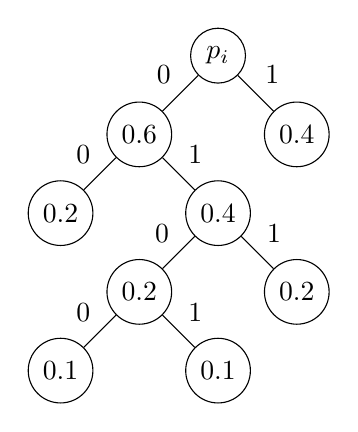
\begin{tikzpicture}
\node[draw, circle] (a) at (0,10) {$p_i$};
\node[draw, circle] (b) at (-1,9) {0.6};
\node[draw, circle] (c) at (1,9) {0.4};
\node[draw, circle] (d) at (0,8) {0.4};
\node[draw, circle] (e) at (-2,8) {0.2};
\node[draw, circle] (f) at (1,7) {0.2};
\node[draw, circle] (g) at (-1,7) {0.2};
\node[draw, circle] (h) at (0,6) {0.1};
\node[draw, circle] (i) at (-2,6) {0.1};

\draw (a) -- node[above left] {0} (b) (a) -- node[above right] {1} (c);
\draw (b) -- node[above left] {0} (e) (b) -- node[above right] {1} (d);
\draw (d) -- node[above left] {0} (g) (d) -- node[above right] {1} (f);
\draw (g) -- node[above left] {0} (i) (g) -- node[above right] {1} (h);
\end{tikzpicture}
\end{subfigure}
\begin{subfigure}{0.5\textwidth}
\begin{tabular}{c|c|c}
$i$ & $p_i$ & Codewords \\\hline
1 & 0.4 & 1\\
2 & 0.2 & 00\\
3 & 0.2 & 011\\
4 & 0.1 & 0100\\
5 & 0.1 & 0101
\end{tabular}
\end{subfigure}
\end{figure}
This code has expected length $2.2$, which is less than Shannon-Fano gave.
\begin{theorem}[Huffman, 1952]
Huffman codes are optimal.
\end{theorem}
\begin{proof}
We show this by induction on $m$. The case of $m=2$ is trivial. For $m > 2$, let $c_m$ be a Huffman code for source $X_m$ which takes values $\mu_1, \ldots, \mu_m$ with probabilities $p_1 \geq \ldots \geq p_m$. Then $c_{m-1}$ is constructed from a Huffman code $c_{m-1}$ for values $\mu_1, \ldots, \mu_{m-1}, \nu$ with probabilities $p_1, \ldots, p_{m-2}, p_{m-1}+p_m$.

Observe that $\E S_m = \E S_{m-1} + p_{m-1} + p_m$ by construction of $c_m$ from $c_{m-1}$.

Now let $c_m'$ be an optimal code for $X_m$. Without loss of generality, we may take $c_m'$ to be prefix-free and the last two codewords of $c_m'$ have maximal length and differ only in the last digit (see \textbf{3.2} below). Say $c_m'(\mu_{m-1}) = y0, c_m'(\mu_m) = y1$ for some $y \in \{0, 1\}^\ast$.

Let $c_{m-1}'$ be the prefix free code for $X_{m-1}$ given by $c_{m-1}'(\mu_i) = c_m'(\mu_i), c_{m-1}'(\nu) = y$.

Then the expected word length is $\E S_m' = \E S_{m-1}' + p_{m-1} + p_m \geq \E S_{m-1} + p_{m-1} + p_m = \E S_m$ by the inductive hypothesis, and so $c_m$ is optimal.
\end{proof}
\begin{lemma}
Suppose messages $\mu_1, \ldots, \mu_m$ are sent with probabilities $p_1,\ldots, p_m$, with an optimal code $c$ with word lengths $\ell_1, \ldots, \ell_m$. Then:
\begin{enumerate}
\item If $p_i > p_j$ then $\ell_i \leq \ell_j$.
\item Among all codewords of maximal length, there are two that differ only in the last digit.
\end{enumerate}
\end{lemma}
\begin{proof}
Otherwise, modify $c$ by swapping the $i\th$ and $j\th$ codewords, or deleting the last letter of each codeword of maximal length. The modified code is still prefix-free but has shorter expected word length, contradicting optimality of $c$.
\end{proof}
\section{Joint Entropy}
If $X,Y$ are random variables with value in $\mathcal{A}$ and $\mathcal{B}$. Then $(X,Y)$ is also a random variable with entropy $H(X,Y)$, the \emph{joint entropy} of $X,Y$.
\begin{align*}
H(X,Y) = -\sum_{x \in \mathcal{A}} \sum_{y \in \mathcal{B}} \P(X=x, Y=y)\log \P(X=x, Y=y)
\end{align*}
We can of course generalise this to any finite number of random variables. We will use Gibb's (\textbf{2.1}) to prove:
\begin{lemma}
Let $X,Y$ be random variables taking values in $\mathcal{A}, \mathcal{B}$. Then:\begin{align*}
H(X,Y) \leq H(X) + H(Y)
\end{align*}
with equality if and only if $X$ and $Y$ are independent.
\end{lemma}
\begin{proof}
Let $\mathcal{A} = \{x_1, \ldots, x_m\}, \mathcal{B} = \{y_1, \ldots, y_n\}$. Set $p_{ij} = \P(X=x_i, Y=y_i), p_i = \P(X=x_i), q_i = \P(Y=y_i)$. Then Gibb's inequality with $\{p_{ij}\}$ and $\{p_iq_j\}$ gives:
\begin{align*}
-\sum_{i,j} p_{ij}\log p_{ij} \leq -\sum_{i,j} p_{ij}\log(p_iq_j) &= -\sum_i\left(\sum_j p_{ij}\right) \log p_i - \sum_j \left(\sum_i p_{ij}\right) \log q_j\\
&= -\sum_i p_i \log p_i -\sum_j q_j \log q_j
\end{align*}
i.e. $H(X,Y) \leq H(X) + H(Y)$, with equality if and only if $p_{ij} = p_i q_j$ for all $i, j$, i.e. when $X,Y$ are independent.
\end{proof}

\hspace*{-1em}\underline{Example:} Let $X$ be a random variable that takes $D$ values with probability $\frac1D$. Then $H(X) = \log_2(D)$. Suppose $X_1, \ldots, X_N$ are i.i.d. with the same distribution as $X$. Then $H(X_1, \ldots, X_N) = N \log_2 D$.

\section{Error Correcting Codes}
\subsection{Noisy Channels and Hamming's Code}
A \emph{binary [n,m]-code} is a subset $C \subseteq \{0,1\}^n$ of \emph{size} $m = |C|$, \emph{length} $n$. The elements of $C$ are called \emph{codewords}. We use an $[n,m]$-code to send one of $m$ messages through a binary symmetric channel, making $n$ uses of the channel. Clearly $1 \leq m \leq 2^n$, so $0\leq \frac{1}{n}\log m \leq 1$. If $|C| = 1$ then $\rho(C) = 0$, and if $C= \{0,1\}^n$ then $\rho(C) = 1$.

For $x, y \in \{0,1\}^n$, the \emph{Hamming distance} $d(x,y) = |\{i:1\leq i\leq n, x_i \neq y_i \}|$, i.e. the number of positions where $x$ and $y$ differ.

We have three possible decoding rules:
\begin{enumerate}
\item The \emph{ideal observer} decoding rule decodes $x \in \{0,1\}^n$ as $c\in C$ maximising $\P(c$ sent$|x$ received$)$.
\item Then \emph{maximum likelihood} decoding rule decodes $x \in \{0,1\}^n$ as $c\in C$ maximising $\P(x$ received$|c$ sent$)$.
\item The \emph{minimum distance} decoding rule decodes $x \in \{0,1\}^n$ as $c\in C$ minimising $d(x,c)$.
\end{enumerate}

\begin{lemma}
\item
\begin{enumerate}
\item If all the messages are equally likely, then 1. and 2. agree.
\item If $p < \frac{1}{2}$, then 2. and 3. agree.
\end{enumerate}
\end{lemma}
\begin{proof}
\item
\begin{enumerate}
\item By Bayes' Rule:
\begin{align*}
\P(c\sent |x \received) = \frac{\P(c \sent)}{\P(x\received)}\P(x\received|c\sent)
\end{align*}
\end{enumerate}
By Hypothesis, $\P(c\sent)$ is independent of $c \in C$, and so for fixed $x$, maximising $\P(c\sent|x\received)$ is the same as maximising $\P(x\received|c\sent)$.

\item Let $r = d(x,c)$. Then $\P(x\received|c\sent) = p^r(1-p)^{n-r} = (1-p)^n\left(\frac{p}{1-p}\right)^r$. Since $p < \frac12$, $\frac{p}{1-p} < 1$, and so maximising $\P(x\received|c\sent)$ is the same as minimising $d(x, c)$.
\end{proof}

For instance, suppose $000$ is sent with probability $\frac{9}{10}$, and $111$ with probability $\frac{1}{10}$, through a binary symmetric channel with error probability $\frac14$. If we receive $110$, the ideal receiver computes $\P(000\sent|110\received)=\frac34; \P(110\sent|110\received)=\frac14$, and so decodes it as $000$. But the minimum distance (and so maximal likelihood) code is $111$. Henceforth, we will decide to use minimal distance decoding. 

Note that minimal distance decoding can be expensive in terms of time and storage if $|C$ is large, and we also need to specify a convention in the case of a tie (e.g. make a random choice, request the message again).

A code is \emph{d-error detecting} if changing up to $d$ digits in each codeword can never produce another codeword. It is \emph{e-error correcting} if, knowing that $x \in \{0,1\}^n$ differs from some codeword in at most $e$ places, we can deduce uniquely what the codeword is.

\hspace*{-1em}\underline{Examples}
\begin{enumerate}
\item A \emph{repetition code} of length $n$ has codewords $00\ldots0, 11\ldots1$. This is an $[n,2]$-code. It is $(n-1)$ error detecting and $\floor{\frac{n-1}{2}}$-error correcting. But the information rate is only $\frac1n$.
\item A \emph{simple parity check code} or \emph{paper tape code}: identify $\{0,1\}$ with $\F_2$ (i.e. arithmetic modulo 2), and let $C = \{(x_1,\ldots, x_n)\in \{0,1\}^n : \sum x_i = 0\}$. This is an $[n, 2^{n-1}]$-code. It is 1-error detecting, but cannot correct errors. Its information rate is $\frac{n-1}{n}$.
\item \emph{Hamming's Original Code} is a $2$-error detecting and 1-error correcting binary [7,16]-code:
\begin{align*}
C = \left.\begin{cases} & c_1+c_3+c_5+c_7 = 0\\ c \in \F_2^7 : & c_2+c_3+c_6+c_7 = 0\\ &c_4+c_5+c_6+c_7 = 0\end{cases}\right\}
\end{align*}
\end{enumerate}
The bits $c_3,c_5,c_6,c_7$ are arbitrary and $c_1, c_2, c_4$ are forced. The information rate is $\frac47$.

Given $x \in \F_2^7$, we form the \emph{syndrome} $z = (z_1,z_2,z_4) \in \F_2^7$, where $z_1 = x_1+x_3+x_5+x_7,$ $z_2 = x_2+x_3+x_6+x_7,$ $z_4 = x_4+x_5+x_6+x_7$. If $x \in C$ then $z = (0,0,0)$. If $d(x,c) = 1$ for some $c \in C$ then $x_i$ and $c_i$ differ for $i = z_1 + 2z_2 + 4z_4$.




\end{document}